\documentclass[8pt]{extarticle}
\usepackage{amsmath, extsizes, enumitem, graphicx, amssymb}
\usepackage[a4paper, margin=0.5cm]{geometry}

\begin{document}
\subsubsection*{\underline{Probability}}
\begin{itemize}
    \item \textbf{Probability of events}: $P(\Omega)=2^{|\Omega|}$, where $P(\Omega)$ is the set
    of all events
    \item \textbf{Uniform distribution}: Every outcome is the same: size of event divided by size of sample space $\Omega$
    ($P(\text{event})=\frac{|\text{event}|}{|\Omega|}$)
    \item \textbf{Non-uniform distribution}: Different outcomes 
    (e.g. $P(\text{heads})=\frac{1}{3}; P(\text{tails})=\frac{2}{3}$)
    \item \textbf{Condition probability}: $P(A|B)=\frac{P(A\cap B)}{P(B)}$ ($P(A|B)$ not defined 
    if $P(B)=0$)
    \item \textbf{Independence}
    \begin{itemize}
        \item A is \underline{attracted} to B if $P(A|B)>P(A)$
        \item A is \underline{repelled} by B if $P(A|B)<P(A)$
        \item A is \underline{indifferent} to B if $P(A|B)=P(A)$
        \item A and B are independent if $P(A\cap B)=P(A)\times P(B)$
        \item \textbf{Mutual Independence}: (e.g. $k=3\rightarrow$ 3 events: $A_1,A_2,A_3$) 
        \begin{itemize}
            \item $P(A_1\cap A_2)=P(A_1)\times P(A_2)$
            \item $P(A_1\cap A_3)=P(A_1)\times P(A_3)$
            \item $P(A_2\cap A_3)=P(A_2)\times P(A_3)$
            \item $P(A_1\cap A_2\cap A_3)=P(A_1)\times P(A_2)\times P(A_3)$
        \end{itemize}
        \item \textbf{Pairwise Independence}: (e.g. $k=3\rightarrow$ 3 events: $A_1,A_2,A_3$)
        \begin{itemize}
            \item $P(A_1\cap A_2)=P(A_1)\times P(A_2)$
            \item $P(A_1\cap A_3)=P(A_1)\times P(A_3)$
            \item $P(A_2\cap A_3)=P(A_2)\times P(A_3)$
        \end{itemize}
    \end{itemize}
    \item \textbf{Expected Value}: $E[X]=\displaystyle\sum_{\sigma\in\Omega} P(\sigma)\times X(\sigma)$ 
    (\textbf{Conditional Expectation}: $E[X|B]=\displaystyle\sum_{\sigma\in\Omega} P_B(\sigma)\times X(\sigma)$)
    \item \textbf{Variance}: $var(X)=E[X^2]-E[X]^2$
    \item \textbf{Standard Deviation}: $\sigma(X)=\sqrt{var(X)}$
    \item \textbf{Inequalities}
    \begin{itemize}
        \item \textbf{Basic}: $P(X\geq a)\leq \frac{E[X]}{a}$
        \item \textbf{Markov}: $a\in\mathbb{R}$ such that $a>0$, $P(|X|\geq a)\leq \frac{E[|X|]}{a}$
        \item \textbf{Chebyshev}: $a\in\mathbb{R}$ such that $a>0$, $P(|X|\geq a)\leq \frac{E[X^2]}{a^2}$
        \item \textbf{Cantelli}: $a\in\mathbb{R}$ such that $a>0$, $P(X-E[X]\geq a)\leq \frac{var(X)}{a^2+var(X)}$
        \item \textbf{Chernoff}: $P(X\geq(1+\theta)pn)\leq e^{-\frac{\theta^2}{3}pn}$
    \end{itemize}
\end{itemize}

\newpage
\subsubsection*{\underline{Many-One Reductions}}
\begin{itemize}
    \item A many-one reduction from $L_1$ to $L_2$ is a total function $f:\Sigma_1^\star\rightarrow
    \Sigma_2^\star$. Following properties must be satisfied:
    \begin{enumerate}
        \item For every string $w\in\Sigma_1^\star,w\in L_1$ iff $f(w)\in L_2$
        \item $f$ is computable
    \end{enumerate}
    \item Meaning, $L_1$ is many-one reducible to $L_2$ ($L_1\preceq_m L_2$)
    \item \textbf{Example 1}: Suppose $L_1$ is undecidable and that $x_{yes},x_{no}\in\Sigma_2^\star$ such 
    that $x_{yes}\in L_2$ and $x_{no}\notin L_2$. Consider the total function $g:\Sigma_1^\star\rightarrow
    \Sigma_2^\star$ 
    $$g(w)= \left\{ \begin{array}{rcl}
        x_{yes} & \mbox{if} & w\in L_1 \\
        x_{no} & \mbox{if} & w\notin L_1
    \end{array}\right.$$
    \item \textbf{Answer}: Function $g$ is \textbf{not} a many-one reduction from $L_1$ to $L_2$
    \begin{itemize}
        \item Function $g$ is not computable. Can be shown by proof of contradiction - that is, 
        assuming that $g$ \textit{is} computable.
    \end{itemize}
    \item \textbf{Example 2}: Suppose that next, $L_1=\emptyset$ and $L_1\neq\Sigma_1^\star$. 
    Consider a total function $h:\Sigma_1^\star\rightarrow\Sigma_2^\star$ such that $h(w)=x_{yes}$
    \item \textbf{Answer}: Not a many-one reduction from $L_1$ to $L_2$
    \begin{itemize}
        \item Since $L_1\neq\Sigma_1^\star$ there exists a string $z\in\Sigma_1^\star$ such that 
        $z\notin L_1$. However, $h(z)=x_{yes}\in L_2$, so the requirement "for all $w\in\Sigma_1^\star,
        w\in L_1\text{ iff } h(w)\in L_2$ is not satisfied. 
    \end{itemize}
\end{itemize}
\begin{figure}
    \begin{minipage}{0.333\textwidth}
        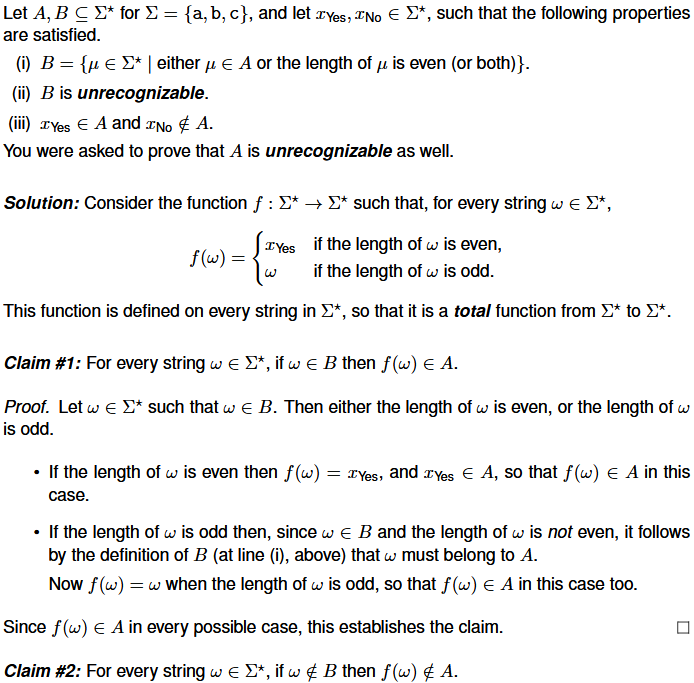
\includegraphics[width=\linewidth]{reduction1.png}
    \end{minipage}\hfill
    \begin{minipage}{0.333\textwidth}
        \centering
        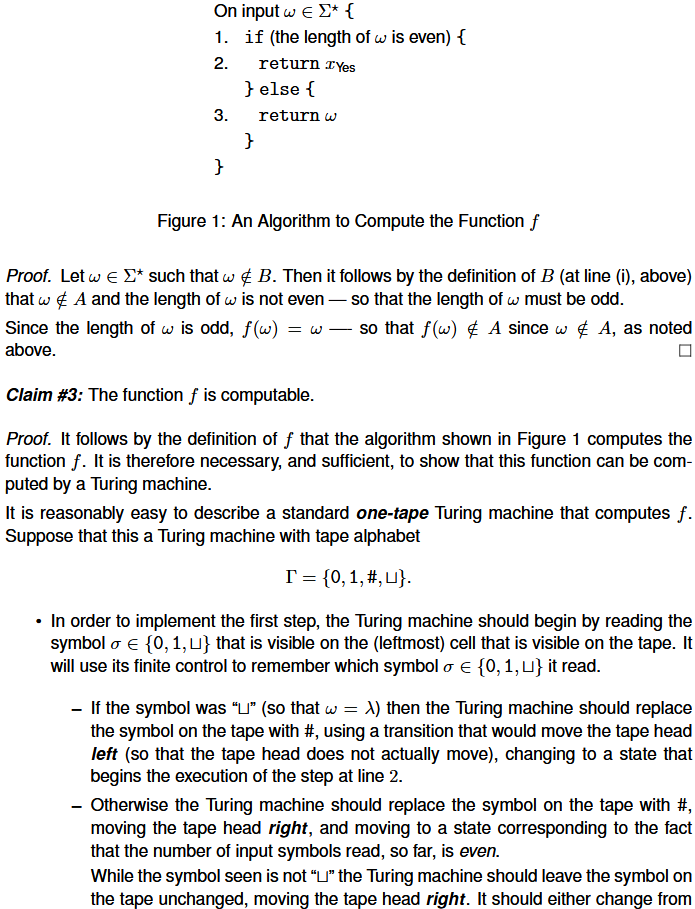
\includegraphics[width=\linewidth]{reduction2.png}
    \end{minipage}\hfill
    \begin{minipage}{0.333\textwidth}
        \centering
        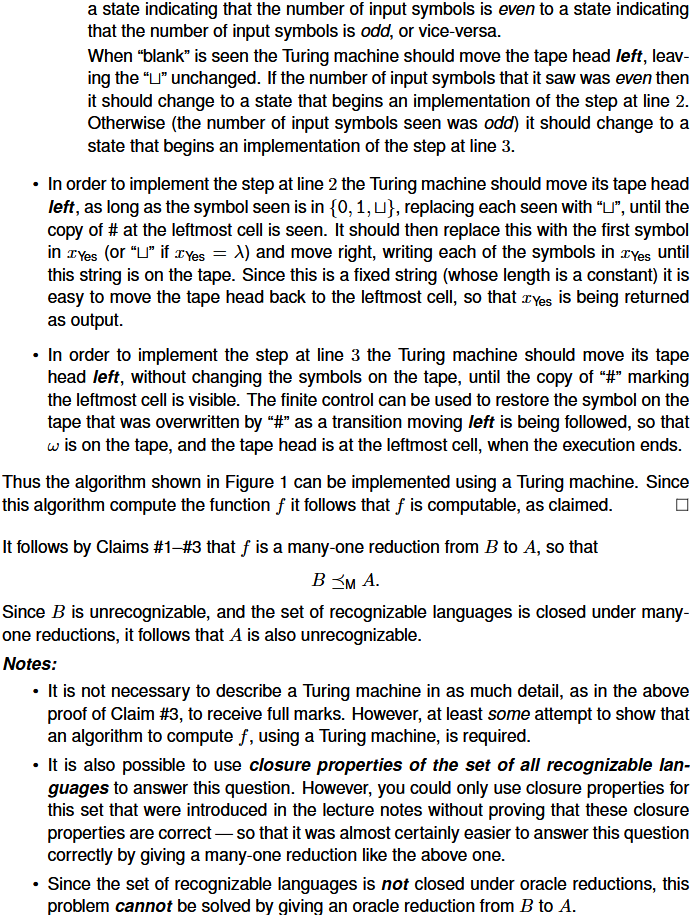
\includegraphics[width=\linewidth]{reduction3.png}
    \end{minipage}\hfill
\end{figure}

\subsubsection*{\underline{DFA}}
\begin{enumerate}[label=(\alph*)]
    \item \textbf{DFA}
    \item \textbf{Describe set of strings corresponding to states}
    \begin{itemize}
        \item Prompt: $L=\{w\in\Sigma^\star|\text{$w$ ends with "ab" and the copies of "a" is even}\}$
        \item Format: $S_{\lambda,even}=\{w\in\Sigma^\star|\text{$w$ does not end with "a" or "ab", and copies of "a" is even}\}$
        correponds to state $q_0$
        \item Do it for every state!
    \end{itemize}
    \item \textbf{Claims needed to verify transitions out of start state}
    \begin{itemize}
        \item $\{w\cdot a|w\in S_0\}\subseteq S_{od}$
        \item $\{w\cdot b|w\in S_0\}\subseteq S_0$
        \item $\{w\cdot c|w\in S_0\}\subseteq S_0$
    \end{itemize}
    \item \textbf{Proof that the transition out of the start state} (for some symbol) 
    \textbf{is correct and well-defined} (e.g. \textit{b} in $S_{\lambda,ev}$)
    \begin{itemize}
        \item Let $w\in S_{\lambda,ev}$ - so that $w$ does not end with "a" or "ab" and the copies 
        of "a" is even. Now, string $w\cdot b$ certainly cannot end with "a". In order for the string 
        to end with "ab", $w$ must end with "a".
        \item String $w\cdot b$ has as many copies of "a" as $w$ does, so number of copies of "a" in
        $w\cdot b$ is even. 
    \end{itemize}
    \item \textbf{Additional claims} (format)
    \begin{enumerate}[label=(\roman*)]
        \item Every string must belong to exactly \textbf{one} of the sets - that is, exactly one of
        (set of states here - e.g. $S_0, S_a$)
        \item $\lambda\in S_0$ because it is the start state
        \item Need to prove that $S\cap L=\emptyset$ for every set not in the set $F$ of accepting states (e.g. $S_{\lambda,ev}\cap L=\emptyset$)
        \item Need to prove that $S\subseteq L$ for every set that belongs to F (e.g. $S_{ab}\subseteq L$)
    \end{enumerate}

\end{enumerate}

\end{document}
